\section{Setup}
\begin{frame}
	\centering
	\includegraphics{./figures/setup.pdf}
\end{frame}

% \begin{frame}
% 	\begin{columns}
% 		\column{.5\textwidth}
% 		\centering
% 		\includegraphics[width=\textwidth]{figures/trap nist schematic.png}

% 		\column{.5\textwidth}
% 		\centering
% 		\includegraphics[width=\textwidth]{figures/trap nist.png}
% 	\end{columns}
% 	\customcite[]{nist_infrared_2024}
% \end{frame}

% \begin{frame}
% 	\begin{columns}
% 		\column{.5\textwidth}
% 		\centering
% 		\includegraphics[width=\textwidth]{figures/detector reflectance.png}

% 		\column{.5\textwidth}
% 		\centering
% 		\includegraphics[width=\textwidth]{figures/trap efficency.png}
% 	\end{columns}
% 	\customcite[]{fox_trap_1991}
% \end{frame}

\begin{frame}
	\begin{columns}
		\column{.5\textwidth}
		\centering
		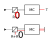
\includegraphics{figures/setup single monochromator.pdf}

		\column{.5\textwidth}
		Assuming MC is symmetric $\eta_\rightarrow = \eta_\leftarrow$:\\
		\begin{align*}
			T &= \eta\; L \\
			R &= \eta^2\;L\\
			\rightarrow \eta &= R /T
		\end{align*}
	\end{columns}
\end{frame}